\documentclass{article}
\usepackage[top=1in, bottom=1in, left=1in, right=1in]{geometry}
\usepackage{amsmath,cite}
\usepackage{graphicx}
\usepackage{subcaption}
\usepackage{times, epsfig, graphicx,url, bm}
\usepackage{amssymb}
\usepackage{epstopdf}
\usepackage{tikz}
\usetikzlibrary{bayesnet}

\DeclareMathOperator*{\argmax}{arg\,max}


% Title.
% ------
\title{Dictionary Prior $\mathrm{P}(\mathbf{W})$}
\author{
Dawen Liang \\
\texttt{daliang@adobe.com}
} \date{}

\begin{document}
%
\maketitle
%

\section{Source-filter model (version 1)}
\begin{figure}[ht]
  \centering
      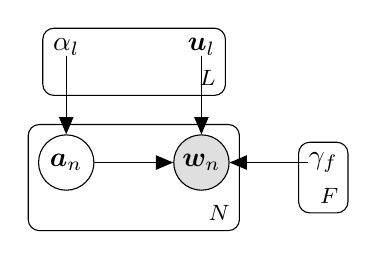
\begin{tikzpicture}

  % Define nodes
  \node[obs] 			(w) {$\bm{w}_n$};
  \node[const, right=of w] (s) {${\gamma}_f$};
  \node[latent, left=of w] (a) {$\bm{a}_n$};
  \node[const, above=of w] (u) {$\bm{u}_l$};
  \node[const, above=of a] (alpha) {$\alpha_l$};

  % Connect the nodes
  \edge {a} {w} ; %
  \edge {s} {w};
  \edge {u} {w};
  \edge {alpha}{a};

  % Plates
  \plate {wa} {(w)(a)} {$N$};
  \plate {au} {(alpha)(u)} {$L$};
  \plate {sigma} {(s)} {$F$};

\end{tikzpicture}

  \caption{Version 1}
\label{fig:plate}
\end{figure}

Model formulation:
\[
\bm{w}_t \in \mathbb{R}_{+}^{F} \qquad \bm{a}_t \in \mathbb{R}_{+}^{L} \qquad \bm{u}_l  \in \mathbb{R}_{+}^{F}\\
\]
\begin{align*}
a_{tl} &\sim \Gamma(\alpha_l, \alpha_l)\\
\log {w}_{tf} &\sim \mathcal{N}(\sum_{l=1}^L a_{tl} u_{lf}, 1/\gamma_f)
\end{align*}

Objective:
\begin{align*}
\hat{\mathbf{U}}, \hat{\bm{\alpha}}, \hat{\bm{\gamma}} &= \argmax_{\mathbf{U}, \bm{\alpha}, \bm{\gamma}} \sum_t \log P(\bm{w}_t | \mathbf{U}, \bm{\alpha}, \bm{\gamma})\\
&= \argmax_{\mathbf{U}, \bm{\alpha}, \bm{\gamma}} \sum_t \log \int_{\bm{a}_t} P(\bm{w}_t, \bm{a}_t | \mathbf{U}, \bm{\alpha}, \bm{\gamma}) \mathrm{d} \bm{a}_t
\end{align*}


\section{Variational EM:}
\subsection{E-step}
\begin{itemize}
\item Reparametrize $v_{tf} \equiv \log w_{tf}$ and $\phi_{tl} \equiv \log a_{tl}$.
\item Approximate posterior $P(\bm{a}_t | \mathbf{U}, \bm{w}_t, \bm{\alpha}, \bm{\gamma}) = \prod_{l} q(a_{tl})$, where $q(\log a_{tl}) \equiv q(\phi_{tl}) = \mathcal{N}(\mu_{tl}, \sigma_{tl}^2)$.
\end{itemize}

\subsubsection{Laplace Approximation:} 

\begin{align*}
q(a_{tl}) &\propto \exp \{ (\alpha_l - 1) \log a_{tl} - \alpha_l a_{tl} - \frac{1}{2} \sum_f \gamma_f  \langle (v_{tf} - \sum_k a_{tk} u_{kf})^2 \rangle \}\\
\Rightarrow q(\phi_{tl}) &\propto \exp \biggl\{ \alpha_l  \phi_{tl}  + \exp(\phi_{tl}) \biggl(\sum_f \gamma_f u_{lf} \hat{v}_{tf}^{-l} - \alpha_l\biggl) - \frac{1}{2} \exp(2\phi_{tl}) \sum_f \gamma_f u_{lf}^2  \biggl\}\\
&= \exp\{f(\phi_{tl})\}
\end{align*}
where 
\[
\hat{v}_{tf}^{-l} = v_{tf} - \sum_{k\neq l} \langle \exp(\phi_{tk})\rangle u_{kf}
\]

Search for the local maximum $\hat{\phi}_{tl}$ of $f(\phi_{tl})$:
\begin{align*}
\mu_{tl} &\leftarrow \hat{\phi}_{tl}\\
\sigma_{tl}^2 & \leftarrow -\biggl(\frac{\partial^2 f } {\partial \phi_{tl}^2} (\hat{\phi}_{tl})\biggl)^{-1}
\end{align*}

\subsubsection{Directly optimizing variational bound}

 The variational bound is:
\begin{align*}
\mathcal{L}(\bm{\mu}, \bm{\sigma}) =& \sum_t \biggl\{  \langle \log P(\bm{w}_t, \bm{a}_t | \mathbf{U}, \bm{\alpha}, \bm{\gamma}) \rangle + \sum_l H_q (a_{tl}) \biggl\}
\end{align*}
where
\begin{align*}
 \langle \log P(\bm{w}_t, \bm{a}_t | \mathbf{U}, \bm{\alpha}, \bm{\gamma}) \rangle  \propto & \sum_f \langle -\frac{1}{2} \gamma_f (v_{tf} - \sum_k a_{tk} u_{kf})^2 \rangle + \sum_l  (\alpha_l - 1) \langle \log a_{tl} \rangle - \alpha_l \langle a_{tl} \rangle
\end{align*}
and 
\begin{align*}
H_q (a_{tl}) \propto \frac{1}{2}\log ( \sigma_{tl}^2) + \mu_{tl}
\end{align*}
Furthermore,
\begin{align*}
& \sum_f \langle -\frac{1}{2} \gamma_f (v_{tf} - \sum_k a_{tk} u_{kf})^2 \rangle \\
\propto & \sum_f \frac{1}{2} \gamma_f \biggl\{ 2 v_{tf} \sum_k \langle a_{tk} \rangle u_{kf} -  \langle \big(\sum_k a_{tk} u_{kf}\big)^2 \rangle \biggl\}
\end{align*}

All the expectations can be computed as:
\begin{align*}
&\langle a_{tl} \rangle = \exp(\mu_{tl} + \frac{1}{2} \sigma_{tl}^2)\\
&\langle a_{tl}^2 \rangle = \exp(2\mu_{tl} + 2\sigma_{tl}^2)\\
&\langle \log a_{tl} \rangle = \mu_{tl}
\end{align*}

Therefore, we can optimize $\mathcal{L}$ w.r.t. $\bm{\mu}_l$ and $\bm{\sigma}_l^2$ jointly for $l\in [L]$. The objective function is:
\begin{align*}
\mathcal{L}(\bm{\mu}_l, \bm{\sigma}^2_l) 
\propto \sum_t \biggl\{  \langle a_{tl} \rangle (\sum_f \gamma_f u_{lf} \hat{v}_{tf}^{-l} -\alpha_l) - \frac{1}{2} \langle a_{tl}^2 \rangle \sum_f \gamma_f u_{lf}^2
+ (\alpha_l - 1) \langle \log a_{tl} \rangle  + \frac{1}{2}\log (\sigma_{tl}^2) + \mu_{tl} \biggl\} 
\end{align*}
The gradient of $\mathcal{L}(\bm{\mu}_l, \bm{\sigma}^2_l)$: 
\[
\frac{\partial \mathcal{L}}{\partial \mu_{tl}} = \langle a_{tl} \rangle (\sum_f \gamma_f u_{lf} \hat{v}_{tf}^{-l} - \alpha_l) - \langle a_{tl}^2 \rangle \sum_f \gamma_f u_{lf}^2  + \alpha_l  
\]
\[
\frac{\partial \mathcal{L}}{\partial (\sigma^2_{tl})} = \frac{1}{2} \langle a_{tl} \rangle  (\sum_f \gamma_f u_{lf} \hat{v}_{tf}^{-l} - \alpha_l) - \langle a_{tl}^2 \rangle \sum_f \gamma_f  u_{lf}^2 + \frac{1}{\sigma_{tl}^2}
\]

\subsection{M-step:}

The objective function for M-step is:
\begin{align*}
\mathcal{L}(\mathbf{U}, \bm{\alpha}, \bm{\gamma}) &= \sum_t \langle \log P(\bm{w}_t, \bm{a}_t | \mathbf{U}, \bm{\alpha}, \bm{\gamma}) \rangle \\
&\propto \sum_t  \biggl\{ \frac{1}{2}\sum_f \langle \log \gamma_f - \gamma_f (v_{tf} - \sum_k a_{tk} u_{kf})^2 \rangle + \sum_l \langle \alpha_l \log \alpha_l - \log \Gamma(\alpha_l) + (\alpha_l - 1)\log a_{tl} - \alpha_l a_{tl}  \rangle \biggl\}
\end{align*}

Take the derivative w.r.t. $\mathbf{U}, \bm{\alpha}, \bm{\gamma}$, respectively:
\begin{align*}
\frac{\partial \mathcal{L}}{\partial u_{lf}} &\propto \sum_t \biggl( \langle a_{tl} \rangle \hat{v}_{tf}^{-l} - \langle a_{tl}^2 \rangle u_{lf} \biggl)\\
\frac{\partial \mathcal{L}}{\partial \alpha_l} &\propto  \sum_t \biggl( \log \alpha_l + 1 - \psi(\alpha_l) + \langle \log a_{tl} \rangle - \langle a_{tl} \rangle \biggl)\\
\frac{\partial \mathcal{L}}{\partial \gamma_f} &\propto \sum_t \frac{1}{\gamma_f} -  \biggl(v_{tf}^2 - 2 v_{tf}  \sum_k \langle a_{tk} \rangle u_{kf} +  \langle (\sum_k a_{tk} u_{kf})^2 \rangle \biggl)
\end{align*}
where
\begin{align*}
\langle (\sum_k a_{tk} u_{kf})^2 \rangle = \sum_k \langle a_{tk}^2 \rangle u_{kf}^2 + (\sum_k \langle a_{tk} \rangle u_{kf})^2 - \sum_k \langle a_{tk}\rangle ^2 u_{kf}^2
\end{align*}

Note that for $\gamma_f$, closed form update is available:
\begin{equation*}
\gamma_f^{-1} = \frac{1}{T}\sum_t \biggl(v_{tf}^2 - 2 v_{tf}  \sum_k \langle a_{tk} \rangle u_{kf} +  \langle (\sum_k a_{tk} u_{kf})^2 \rangle \biggl)
\end{equation*}

While for $U$ and $\alpha$, L-BFGS can be applied to find a local optimum. Note that since $\alpha_l > 0$ which can be problematic for numerical solver, we log-transform $\eta_l \equiv \log \alpha_l$ and optimize w.r.t. $\eta_l$, where the derivative can be simply modified by chain rule:
\[
\frac{\partial \mathcal{L}}{\partial \eta_l} = \frac{\partial \mathcal{L}}{\partial \alpha_l} \cdot \frac{\partial \alpha_l}{\partial \eta_l} = \alpha_l \frac{\partial \mathcal{L}}{\partial \alpha_l} 
\]

\end{document}
